

\section{Conclusion and Discussion}
This paper introduces a comprehensive framework designed for modeling data revision patterns and generating distributional projections for the revised variables of interest. The versatility of the proposed framework is noteworthy, as it is applicable to a spectrum of data revision challenges where the sequences of data revisions are both available and sufficiently smooth. The application of our model extends across diverse public health data sources, encompassing CHNG outpatient COVID claims data, Quidel COVID Antigen test data, and confirmed cases data from MA DPH. 

To reiterate, we purposely defined our target of projection to be the quantities of interest reported after a certain number of days (target lag) as opposed to awaiting the eventual finalized version, a process that often unfolds several months later for numerous public health data sources. The metric employed for assessing projection performance is based on the target values, assumed to be sufficiently proximate to the finalized values, rather than relying on the actual finalized values. As expounded in the preliminary section, we consciously opt for a trade-off, sacrificing a degree of accuracy relative to the finalized values in favor of a more expeditious response to pattern changes.

Concerning our evaluation approach, we have embraced a symmetrical perspective to gauge relative errors, wherein we assess the absolute deviation between the log-scale predictions and the actual values. This evaluation methodology is scale-independent, ensuring that it remains unaffected by the magnitude of the values under comparison. This characteristic proves particularly advantageous given the wide range of epidemic quantities across different reference dates and locations. Notably, when the original value approaches zero, the relative error can escalate significantly, introducing sensitivity issues. It is imperative to acknowledge that our chosen method inherently grapples with challenges associated with the application of relative errors, as illustrated in Figure X, where suboptimal projection performance is observed for locations naturally characterized by small target fractions.

our framework excels in delivering precise and timely projections for the target version of epidemic quantities of interest. These projections serve a dual purpose by not only alerting surveillance systems to abrupt changes in data revision patterns but also proving instrumental in epidemic forecasting. The ability to preemptively correct both predictors and responses in forecasting challenges can contribute to timely and accurate forecasts in the realm of epidemic monitoring and response.



 

%% TODO: Not the latest version.  
%% Use log 10 or natural log scale? natural log add the second axis? 
\begin{figure}
    \centering
    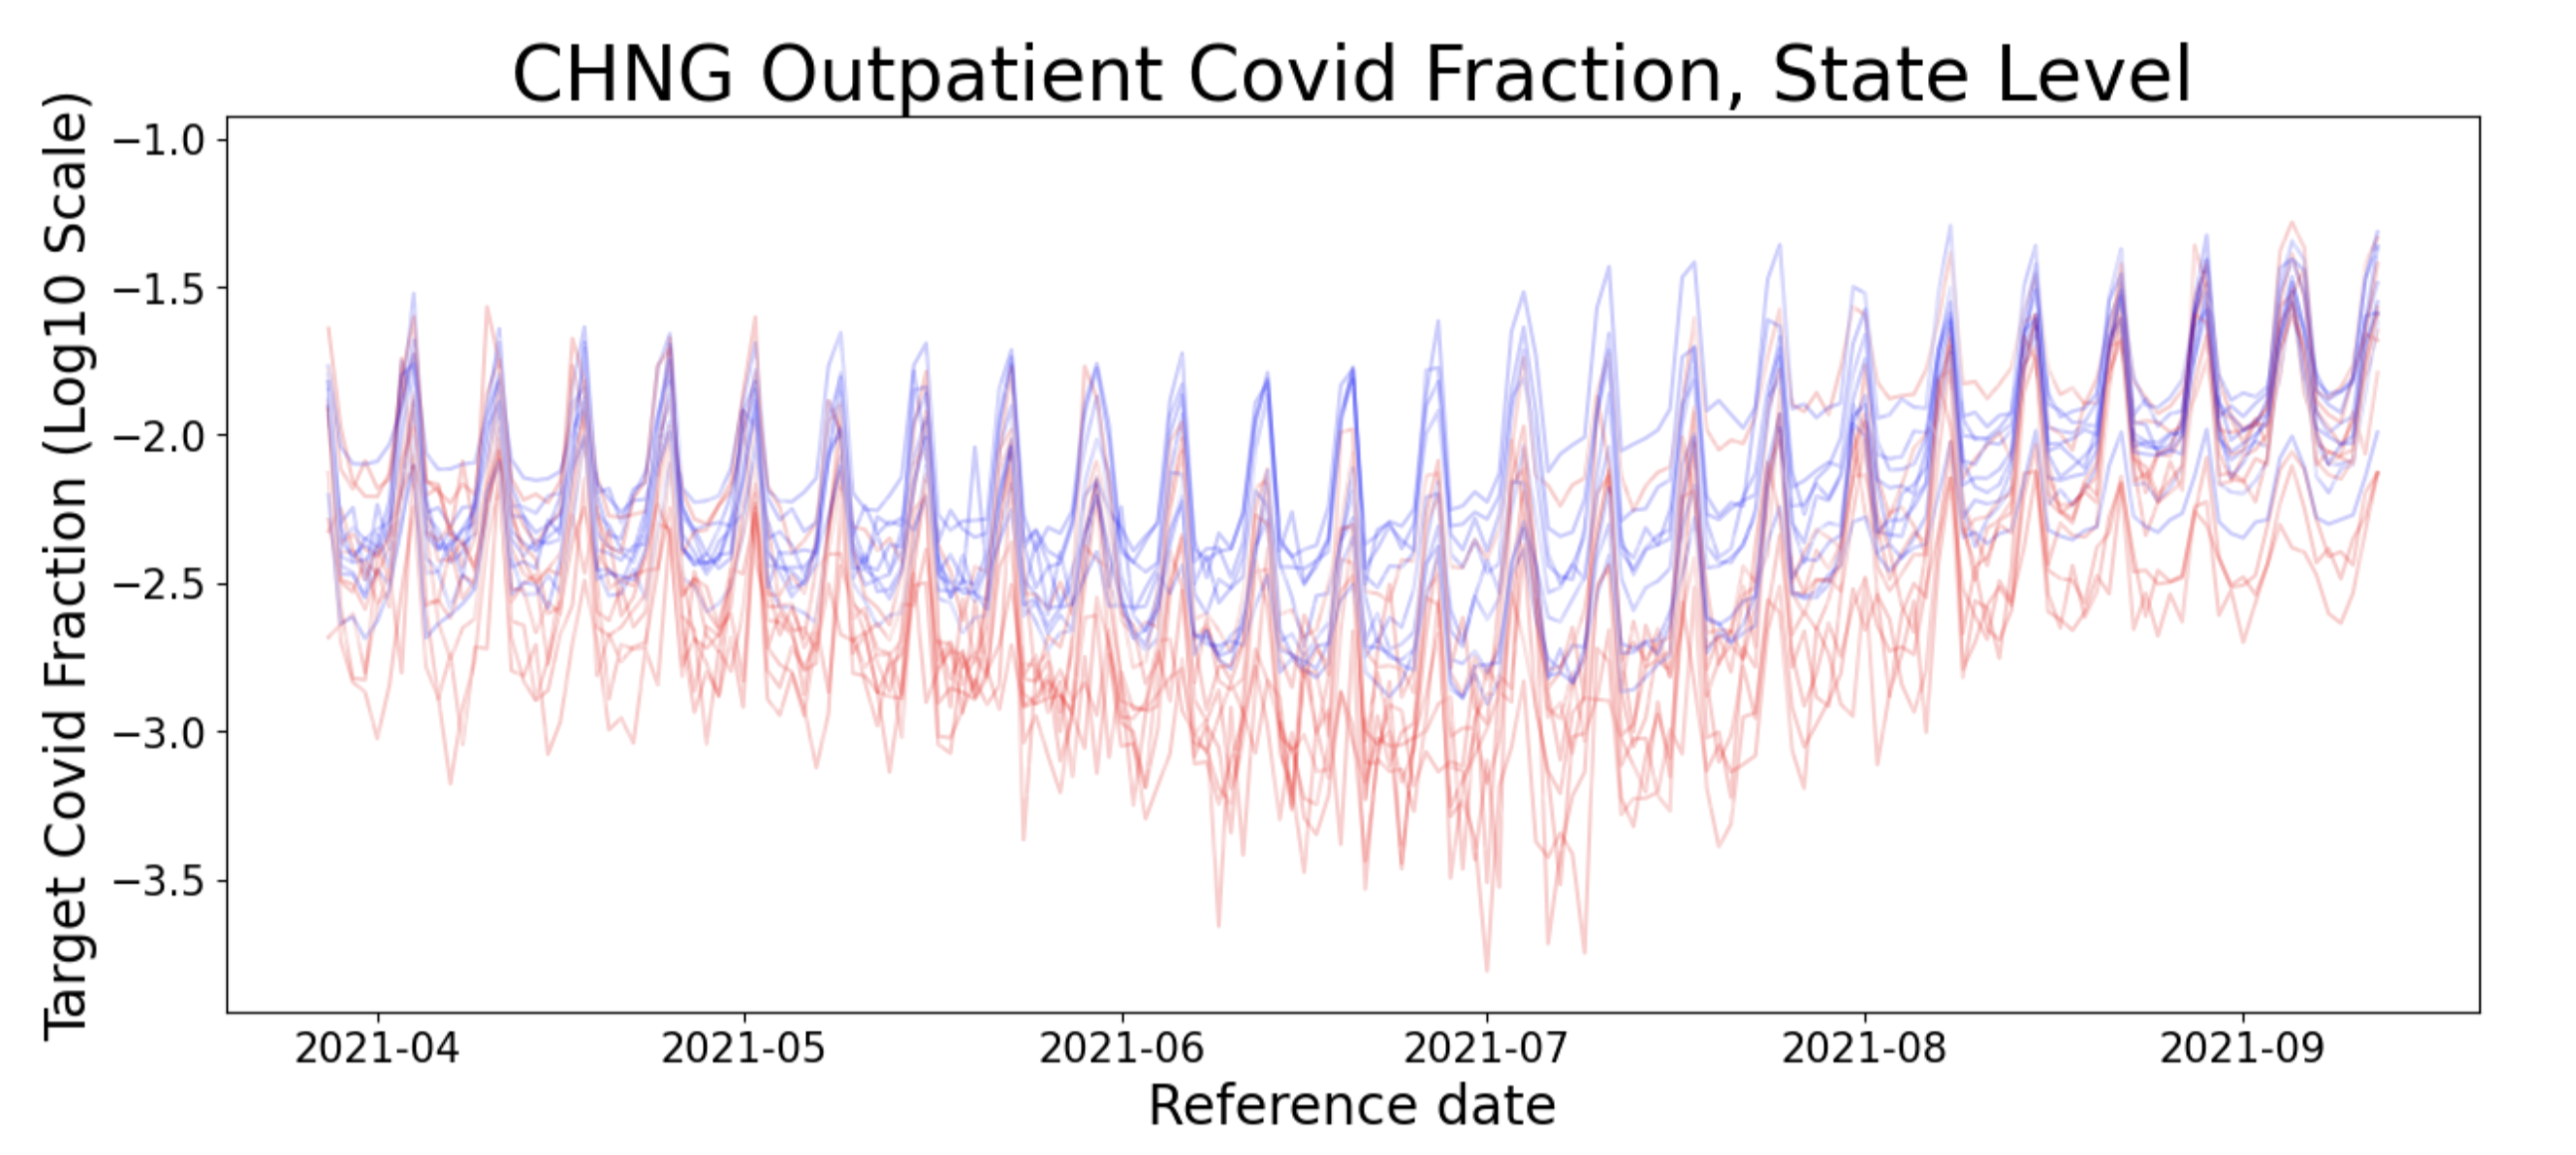
\includegraphics[width=\textwidth]{figs/evl_comparison_states.png}
    \caption{\textit{red lines represent the 10 states with the worst prediction performance while blue lines represent the 10 states with the best prediction performance}}
\end{figure}

%Due to the exponential nature, situations in which models missed the %beginning of upswings are more strongly emphasized while failing to %predict a downturn following a peak is less severely penalized. 
\begin{figure}
    \centering
    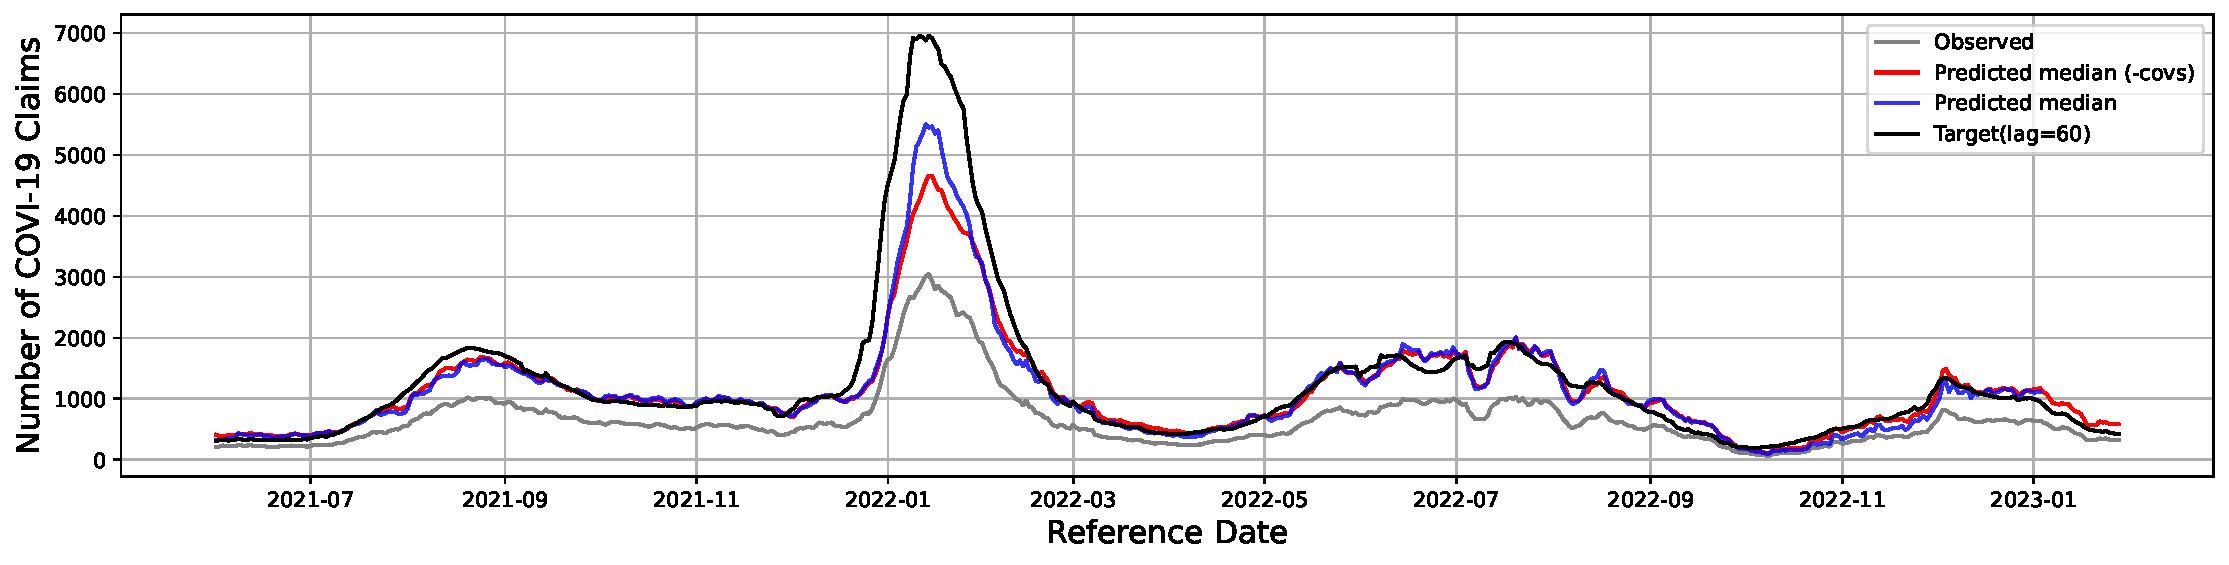
\includegraphics[width=\textwidth]{figs/pred_problem_in_ca.pdf}
    \caption{\textit{the backfill correction}}
\end{figure}

\begin{figure}
    \centering
    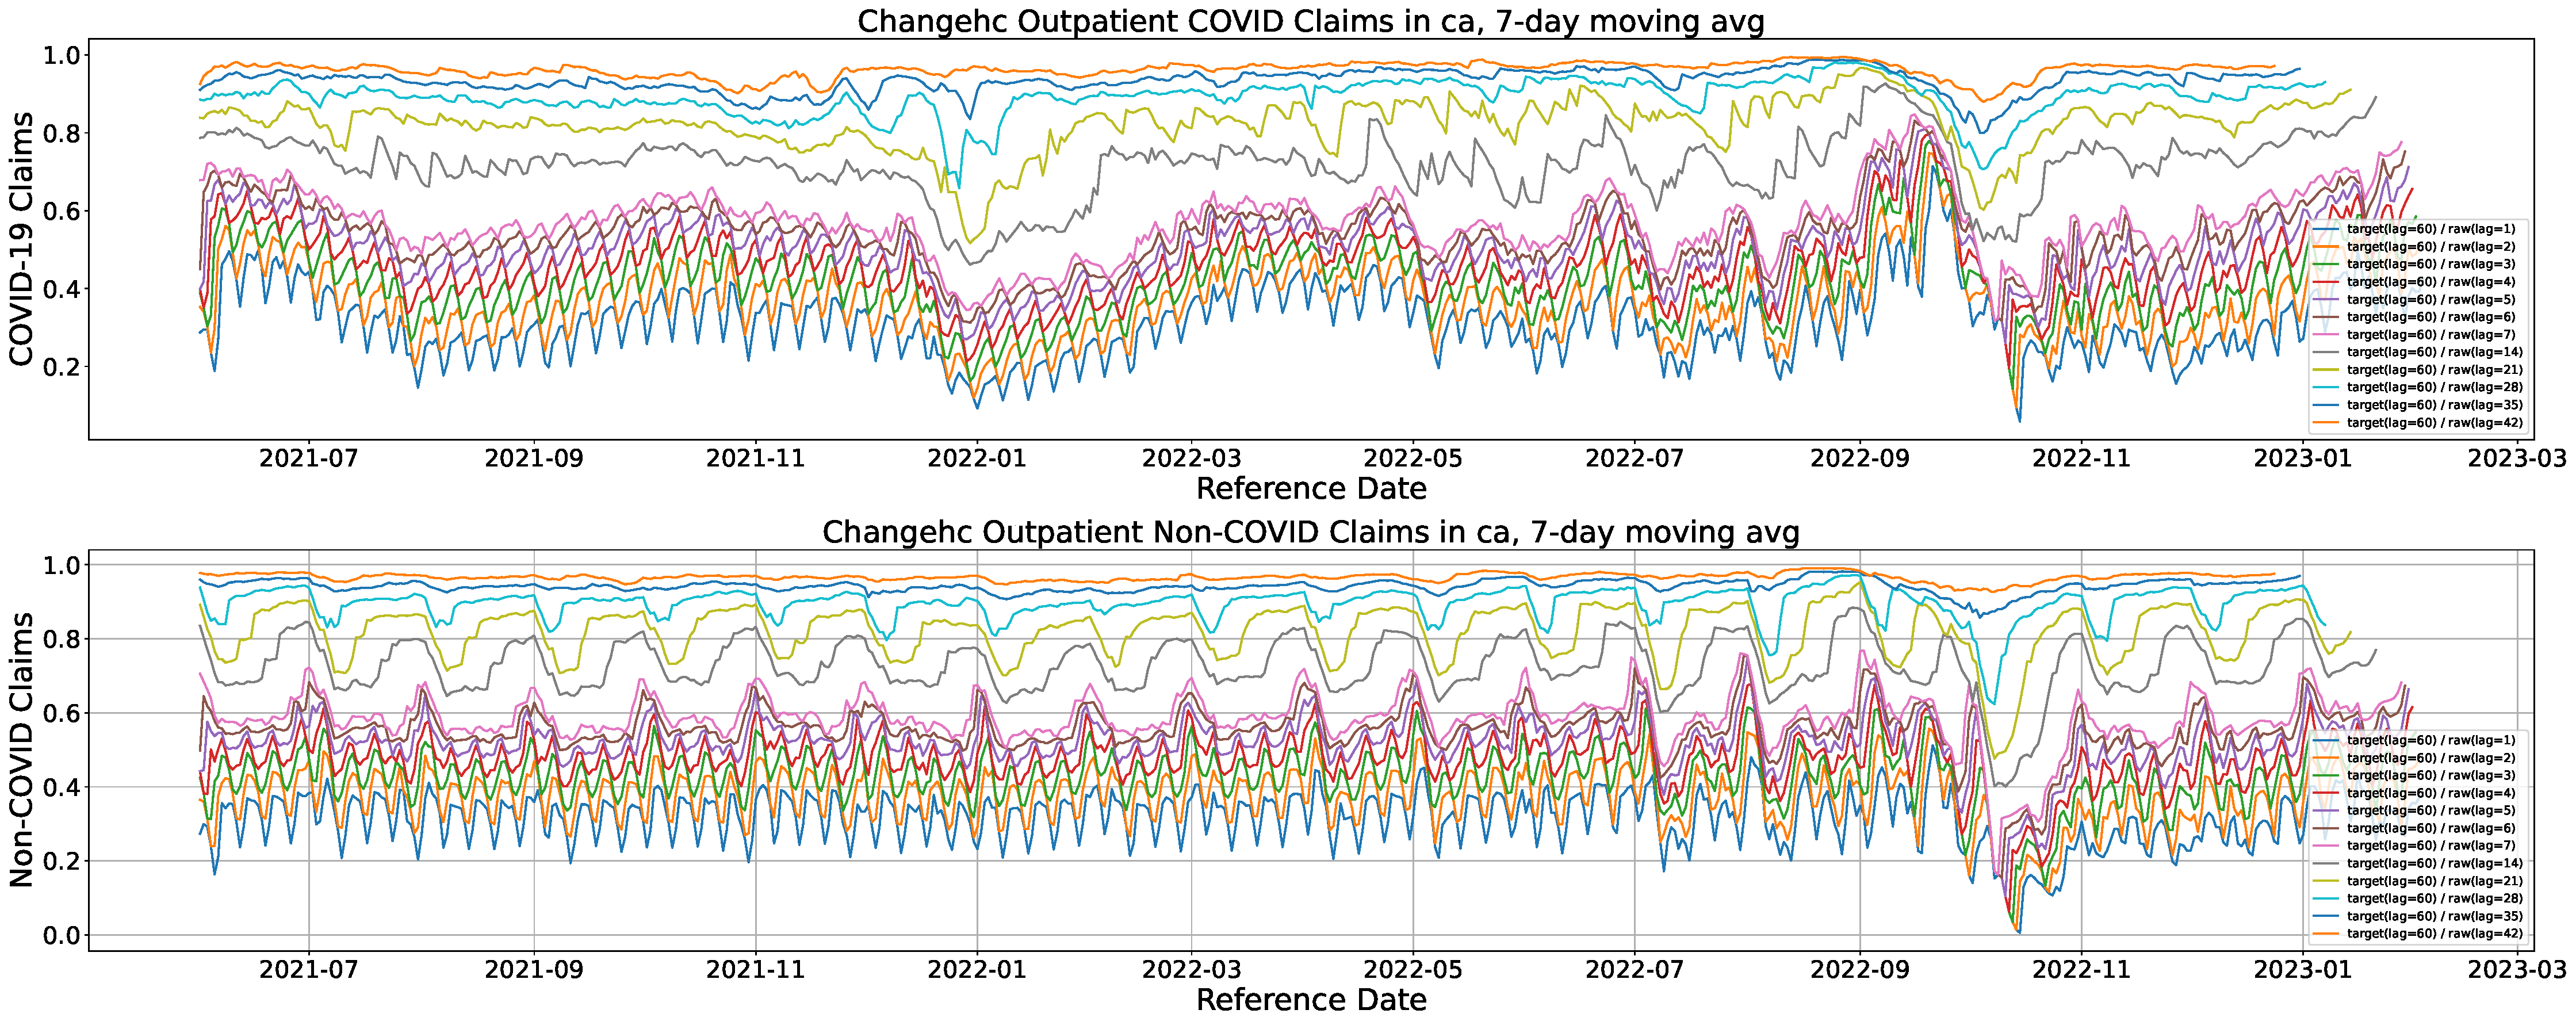
\includegraphics[width=\textwidth]{figs/new_covs_zoom_in.pdf}
    \caption{\textit{the backfill correction}}
\end{figure}



